\chapter{Technical Chapters (change this to something appropriate)}
\textbf{Note: This part of the dissertation will normally be expanded to be a 
\textit{series of chapters}.}

The technical body of the dissertation consists of a number of chapters (just 
one here, but there will usually be more).  Follow a logical structure in how 
you present your work.  This will usually be the phases of the software 
development cycle, the modules of your system, etc. \textbf{\textit{However, 
please do not write your dissertation to read like a diary.}}

Include a chapter demonstrating what you have achieved and how your system is 
used in practice -- for example showing a typical session as a series of pasted 
in screen shots, with an accompanying commentary.

You \textbf{\textit{should}} also include a chapter explaining how you obtained 
feedback from your ``customer'' or potential users of your system, what 
feedback you actually obtained, and your analysis and comments.

\section{First Section}
Subdivide your text into sections, using the \cmd{section} command.

\subsection{First Subsection}
If necessary, also use subsections. Subsections are entered using the 
\cmd{subsection} command (all these heading styles are self-numbering).

%\subsubsection{First Subsubsection}
%If you really need subsubsections, enter these using the \cmd{subsubsection} 
%command. Note that subsubsections in \TeX{} do not display numbers or appear 
%in 
%the Table of Contents (they just show a bold header on its own line).

\subsection{Second Subsection}
And, as required, more subsections.

\section{Bulleted and Numbered Lists}
Note: This section begins with the code 
\texttt{\textbackslash{}section\{Bulleted and Numbered Lists\}} in 
the~\texttt{.tex} file.

Bulleted or numbered lists are entered using the \texttt{itemize} and 
\texttt{enumerate} environments, respectively. An \textbf{environment} in 
\LaTeX{} is a block of code in between a \cmd{begin} and \cmd{end} command. For 
example, the code
\begin{quote}\tt
	\textbackslash{}begin\{itemize\} \\[-0.5em]
	\hspace*{2em}\textbackslash{}item Up \\[-0.5em]
	\hspace*{2em}\textbackslash{}item Down \\[-0.5em]
	\hspace*{2em}\textbackslash{}item Left \\[-0.5em]
	\hspace*{2em}\textbackslash{}item Right \\[-0.5em]
	\textbackslash{}end\{itemize\}
\end{quote}
would produce the following list:
\begin{itemize} \item Up \item Down \item Left \item Right \end{itemize}
The indentation is not necessary (the pdf will look the same even it the 
\texttt{.tex} file does not use indents), but it helps make the code easier to 
read.

If the \texttt{enumerate} environment is used instead, the bullets are replaced 
by numbers. For example, the code
\begin{quote}\tt
	\textbackslash{}begin\{enumerate\} \\[-0.5em]
	\hspace*{2em}\textbackslash{}item Up \\[-0.5em]
	\hspace*{2em}\textbackslash{}item Down \\[-0.5em]
	\hspace*{2em}\textbackslash{}item Left \\[-0.5em]
	\hspace*{2em}\textbackslash{}item Right \\[-0.5em]
	\textbackslash{}end\{enumerate\}
\end{quote}
produces the list
\begin{enumerate} \item Up \item Down \item Left \item Right \end{enumerate}

\section{Figures and Captions}
As an example of a figure, consider Figure \ref{fig:mylovelydiagram}. Captions are 
entered using the \texttt{figure} environment (read the previous section for 
information about environments in general). The code
\begin{quote}\tt
	\textbackslash{}begin\{figure\}[h] \\[-0.5em]
	\hspace*{2em}\textbackslash{}center\textbackslash{}includegraphics[width=12cm]\{image.png\}
	 \\[-0.5em]
	\hspace*{2em}\textbackslash{}caption\{Highly Technical Diagram\} \\[-0.5em]
	\hspace*{2em}\textbackslash{}label\{mylovelydiagram\} \\[-0.5em]
	\textbackslash{}end\{figure\}
\end{quote}
will produce the following figure \textbf{if the file \textit{image.png} is in 
the same folder as your \texttt{.tex} file}.

\begin{figure}[tb]
	\center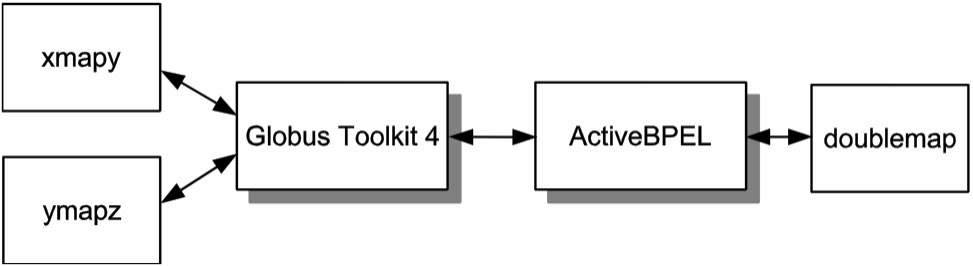
\includegraphics[width=0.6\textwidth]{image.jpg}
	\caption{Highly Technical Diagram}
	\label{fig:mylovelydiagram}
\end{figure}


\begin{figure}[tb]
	\center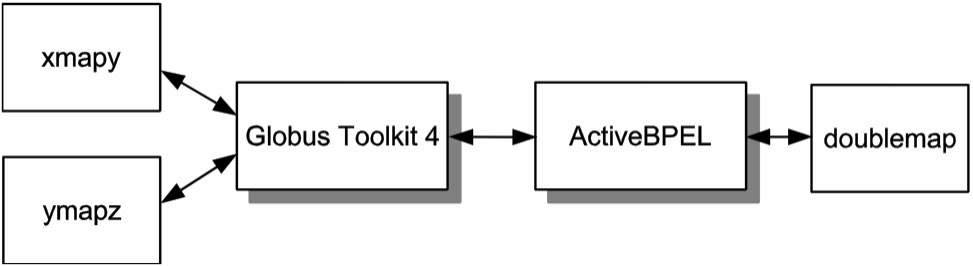
\includegraphics[width=0.6\textwidth]{image.jpg}
	\caption{Highly Technical Diagram two}
	\label{fig:mylovelydiagramtwo}
\end{figure}

The \texttt{[tb]} direction after the beginning of the environment causes the 
figure to be placed ``here'' in the text (at least approximately -- sometimes 
\TeX{} will move the figure slightly if the spacing does not work well in 
exactly the given location). For large figures, use \texttt{[t]} 
or~\texttt{[b]} instead to place the figure at the top or bottom of a page. You 
can also leave off the \texttt{[h]} entirely to have \TeX{} make its best guess 
for where the figure should go.

The \cmd{includegraphics} command puts an image file from your computer into 
your finished pdf. \textbf{If there is no file with the given name in the 
folder with your \texttt{.tex} file, your document will not compile at all.} 
The bracket text \texttt{[width=12cm]} is optional; without it, \TeX{} will use 
the normal size of the image. Sometimes this will be far too large, so it is a 
good idea to specify a width directly.

Figures have automatic numbering, and it is possible to make cross-references 
to figures. The code \cmd{Fig\{mylovelydiagram\}} will create a link to 
\Fig{mylovelydiagram} in the text with the number of that figure. You can 
change the text ``mylovelydiagram'' to be anything you want -- it never appears 
in the final pdf.

\section{Source Code}

To include programming source code in your document, use the 
\texttt{lstlisting} environment. The \LaTeX{} code
\begin{quote}\tt
	\textbackslash{}begin\{lstlisting\}[language=Python, frame=single] 
	\\[-0.5em]
    \hspace*{2em}def factorial(n): \\[-0.5em]
    \hspace*{4em}if n == 0: return 1 \\[-0.5em]
    \hspace*{4em}else: return n * factorial(n-1) \\[-0.5em]
    \textbackslash{}end\{lstlisting\}
\end{quote}
produces the following in the pdf: \\
\begin{lstlisting}[language=Python, frame=single, label={lst:label}, 
caption={Some Python code}]
def factorial(n):
	if n == 0: return 1
	else: return n * factorial(n-1)
\end{lstlisting}
You can change \texttt{language=Python} to \texttt{language=Java}, etc., for 
different programming languages. The \texttt{frame=single} can be removed if 
you do not want the border around your code snippet. See 
\url{https://en.wikibooks.org/wiki/LaTeX/Source_Code_Listings} for syntax 
coloring and other option. You can reference the listing with the command, 
\texttt{\textbackslash{}ref\{lst:label\}}, as in see listing \ref{lst:label}.
